\documentclass[12pt]{iopart}
\usepackage[dvips]{graphicx}
\usepackage{epsfig}
\usepackage{pst-plot}
\usepackage{bm}
\usepackage{setstack}

\eqnobysec
\def\d{\text{d}}
\def\sech{\text{sech}}
\def\Cdot{\!\cdot\!} 
\def\e{\text{e}}
\def\L_2{\L_{2}}
\def\fm{\:\:\mathrm{fm}^{-1}}



\begin{document}
\title[State Dependent Interactions for the Gamow Shell Model.]
      {State Dependent Interactions for the Gamow Shell Model}
      



\author{G Hagen\dag\ddag, M~Hjorth-Jensen\P~and J S Vaagen\ddag}

\address{\dag\ Centre of Mathematics for Applications, University of Oslo, 
N-0316 Oslo, Norway} 
\address{\ddag\ Department of Physics and Technology, University of Bergen,
N-5007 Bergen, Norway}
\address{\P\ Department of Physics and Center of Mathematics for applications, University of Oslo,
N-0316 Oslo, Norway}


\eads{\mailto{gaute.hagen@fys.uio.no},\mailto{morten.hjorth-jensen@fys.uio.no},
  \mailto{jans.vaagen@ift.uib.no} }
\begin{abstract}
A momentum space represenation of the Berggren completeness is used 
in Gamow shell-model calculations of the $^{5-7}$He isotopes. A major
problem in the newly developed Gamow shell model is the extreme 
growth of many-body configurations as the number of valence particles
increases. This problem is addressed using the Lee-Suzuki 
similarity transformation method in the construction of an 
effective two-body interaction. At the converged level the dimensionality 
has been drastically reduced as compared to the full problem. This
offers a promising appoach to the study of weakly bound nuclei.
\end{abstract}

\submitto{\JPG}
\pacs{21.60.Cs, 21.10.-k, 24.10.Cn, 24.30.Gd}

\maketitle
Tanihata's discovery in 1985 \cite{isao} of  spatially
extended nuclei ($^{6,8}$He; $^{11}$Li; $^{11}$Be) at the neutron
dripline, has over the last two decades 
triggered an interest in the study of weakly bound
and resonance phenomena in few-body systems.
A proper description of loosely bound 
nuclei should take into account the coupling of the discrete bound states with the 
continuum of positive scattering states.
This coupling has been neglected in most modern \emph{ab initio} approaches.
The coupling of the external continuum of positive energy states, with the internal 
nuclear states, has for a long time been basic ingredients in nuclear reaction theory. 
Feshbach was the first to formulate a unified description of direct and 
compound nuclear reactions within the projection operator method \cite{feshbach1,feshbach2}. �
He showed that the coupling of the internal with the external environments could 
give rise to compound nuclear states, such as 
multi-channel resonances. As he was the first to 
formulate a general theory of such states, they have become known as Feshbach resonances. 
Also in atomic physics Feshbach resonances
are of great importance. In the early 60's, at the same time of Feshbach, Fano \cite{fano} 
discussed how the mixing of a configuration 
belonging to a discrete spectrum with configurations belonging to a continuous spectrum
gives rise to the phenomena of \emph{autoionization}, which is considered a multi-channel 
resonance or in other words a Feshbach resonance.

Aiming at realistic structure calculations of weakly bound nuclei, a 
unification of standard structure and reaction theory seems to be in place.
If the shell model is to be a reliable theory of such loosely bound or unbound 
systems, a reformulation using a single-particle representation where the continuum is 
properly taken into account has to be searched for. 
In the late 60's Berggren proved that for a finite range potential, 
a finite set of bound and resonant states together with a set of 
non-resonant continuum states form a complete set \cite{berggren}
of bi-orthogonal functions. 
In the Berggren ensemble bound, anti-bound, resonant and the non-resonant continuum
states are treated on equal footing, so  the Berggren basis seems to be
a viable starting point for shell-model calculations of weakly bound and/or 
unbound nuclei.
The  newly developed Gamow shell model is devoted to such an approach, see for example 
references~\cite{michel1,michel2,michel3,liotta,betan,witek1,witek2,roberto,betan2}.
Starting with the discretized single-particle Berggren representation 
\cite{berggren,berggren1,berggren2,berggren3,lind,hagen}, 
a complete anti-symmetrized many-body Berggren basis may be constructed.
This is in full analogy with the standard shell model using a harmonic oscillator basis. 
Expanding the many-body wave functions in this complete set of Berggren Slater 
determinants, allows for an interpretation of exotic multi-particle structures
in terms of single-particle resonances. In this respect,
the Gamow shell model may provide an answer to the question of how exotic 
structures near the dripline, such as multi-particle resonances embedded in the continuum, are formed.

The Gamow shell model is in its early stages, and so there exist  a vast 
area of application and major theoretical and computational challenges to be dealt with.
One of the first challenges and problems encountered in the Gamow shell model, was
the \emph{identification problem}, first addressed in \cite{liotta,betan}.
The physical multi-particle resonances 
will in many cases be embedded in a dense distribution of continuum states, 
depending on the contour in which the continuum states are defined.  
References~\cite{liotta,betan} related this \emph{identification problem} to 
the problem of choosing a contour in the complex $k$-plane which 
in the case of several valence particles selects the physical interesting
states from the dense continuum background. They found that in the two-particle
case, choosing a \emph{square-well} contour makes an identification 
of physical states based on 
inspection of the zeroth order energy surface possible. This solution is
only  applicable in the two-particle case, since even the tree-particle case
the pole configurations get mixed in with the continuum configurations.
In references~\cite{michel2,witek1,witek2} the problem of identifying multi-particle 
resonances was approached from a different angle.
The proposed algorithm is a two step procedure. In the first step 
a diagonalization within the pole space, where all particles are in 
resonant single-particle orbitals, is performed. Secondly a 
diagonalization within the complete configuration space is performed. 
Under the assumption of weak coupling of the pole configurations
with the configurations where at least one particle moves in a continuum orbital, 
the physical states may be picked out unambiguously from the states obtained after a 
full diagonalization, using the criterion of largest overlap with the pole space.
The weak coupling limit may not always be a valid assumption, 
as pointed out in reference~\cite{betan2} 
for the case of $^{11}$Li, the two-particle resonances may
have a larger continuum component as compared to the pole component,
depending on the strength of the residual nucleon-nucleon interaction.
To this end, one may conclude that the \emph{identification problem} has not
been solved generally, and developing an algorithm which picks out 
physical states unambiguously from the dense continuum background is still an open problem.

Another challenge for the Gamow shell model is the \emph{dimensionality problem}, which is the 
main topic of this paper. As the number
of active particles moving in a valence space increases, the 
number of Slater determinants in the many-body Berggren basis increases dramatically. 
This explosion of many-body configurations is in the Gamow shell model approach
even more severe than in the 
standard shell model where only bound states appear. In the Gamow shell model
one has for each partial wave a finite number of non-resonant continuum states which is absent
in the standard shell model. In solving \emph{dimensionality problem}, one has to take advantage of 
effective operator and perturbation method techniques 
typically used and developed for large scale shell-model 
calculations using harmonic oscillator bases. 

In this work we consider as a test case the light 
drip-line nuclei $^{5,6,7}$He, and the formation 
of resonances in these nuclei. 
 These nuclei have also been 
studied with a number of other methods, see for example reference~\cite{jonson}, 
and references therein.
We  construct a single-particle basis using the contour deformation method 
in momentum space, discussed in detail in reference~\cite{hagen}, which is 
used in constructing a complete set of two- and three particle Slater determinants.
Our solution to the \emph{dimensionality problem} is a compromise between the
inspection method used in reference~\cite{liotta,betan} and the overlap
method used in references~\cite{michel2,witek1,witek2}. 
We show that choosing a rotated plus translated contour in the complex
plane, a large portion of the zeroth order many-particle energy surface is free from
complex continuum states. So in this respect an identification based on 
inspection of the zeroth order energy spectrum is possible, by studying
how the two- and three-particle resonances develop as the nucleon-nucleon 
interaction is gradually turned on.
In going beyond two valence particles, we divide the
complete many-body space in two sub-spaces, a model and a complement space. 
In the case of the three-particle resonances in $^7$He, we 
construct an effective interaction at the two-body level in the model space. 
The model space is chosen optimally, and the effective interaction takes into
account the most important many-body correlations, giving a much faster convergence
with increasing model space as compared with the ``bare'' interaction.

The outline of the paper is the following. In section~\ref{sec:formalism} 
we present results of the energy spectra of the $^{5-7}$He isotopes 
using the bare interaction and performing a full diagonalization. 
In section~\ref{sec:suzuki}  the Lee-Suzuki similarity transformation method
is presented, and generalized to complex interactions. A convergence study 
of the ${3/2}^�$ ground state of $^7$He using the bare and the effective interaction 
is given. Section~\ref{sec:conclusion} gives the conclusions of the present study and 
future perspectives and challenges for 
Gamow shell-model calculations.


\section{Gamow Shell-Model calculations of the $^{5-7}$He isotopes.}
\label{sec:formalism}
\subsection{$^5$He single-particle basis using the contour deformation method.}
\label{subsec:helium5}
In reference~\cite{hagen} we studied the contour deformation method applied to 
the momentum space Schr\"odinger equation. It was 
discussed and shown how the specific choices of contours  based on the analytic 
structure of the potential may allow for a unified description of
bound, anti-bound (virtual) and resonant states.
Here, and in reference~\cite{hagen1}, 
CDM is the basic starting point for obtaining a single-particle Berggren basis 
for use in Gamow shell-model calculations. 

The analytically continued Schr\"odinger equation on a general 
inversion symmetric contour takes the form
\begin{equation}
\label{eq:neweq1}
{\hbar^{2}\over 2\mu}k^2\psi_{nl}(k) + {2\over\pi}\int_{C^{+}} 
dq {q}^{2}V_{l}(k,q)\psi_{nl}(q) = E_{nl}\psi_{nl}(k).
\end{equation}
Here both $k$ and $q$ are defined on an inversion symmetric contour $C^+$ in the lower
half complex $k$-plane, resulting in a closed integral equation. 
The eigenfunctions constitute a complete bi-orthogonal set, 
normalized according to the Berggren metric \cite{berggren,berggren1,berggren2,berggren3,lind}, namely
\begin{equation}
\label{eq:unity2}
{\bf 1} = \sum _{n\in \bf{C}}\vert\psi_{nl}\rangle\langle\psi_{nl}^{*}\vert + 
\int_{C^{+}} dk k^2\vert\psi_{l}(k)\rangle\langle\psi_{l}^{*}(k)\vert.   
\end{equation} 
This work uses a single-particle Berggren basis defined
on a rotated plus translated contour, $C_{R+T}^+$, in the complex $k$-plane, 
studied in detail in reference~\cite{hagen}. 
The contour $C_{R+T}^{+}$ is part of the inversion symmetric contour $C_{R+T} = C_{R+T}^{+} + 
C_{R+T}^{-}$ displayed in Fig.~\ref{fig:contour2}.
\begin{figure}[hbtp]
\begin{center}
\resizebox{8cm}{5cm}{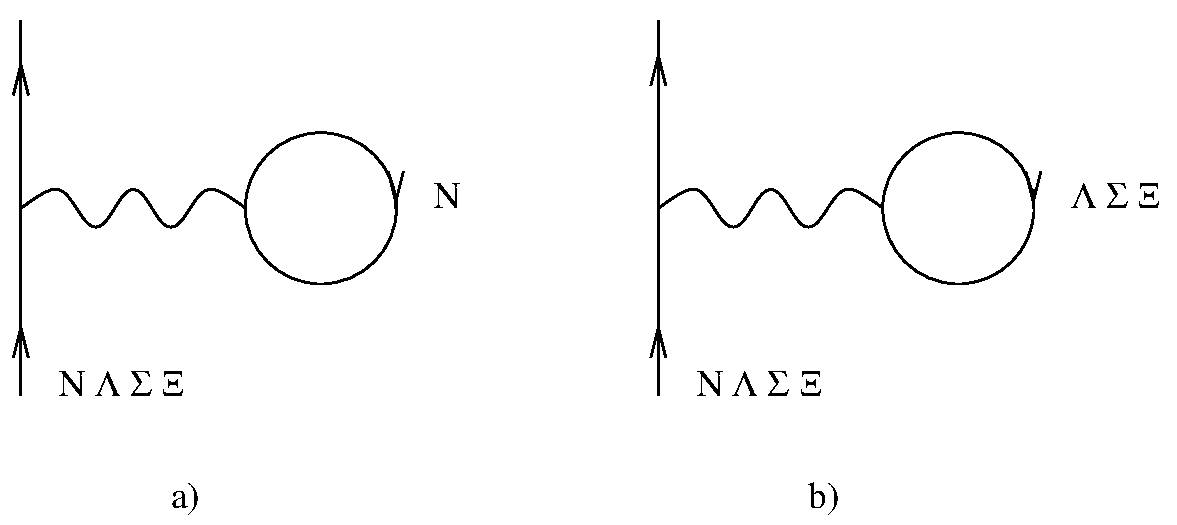
\epsfig{file=fig1.eps}}
\end{center}
\caption{Contour $ C_{R+T}^{+} = L_{1} + L_{2} + L_{3} $ is given 
by the solid line, while
the contour $C_{R+T}^{-} $ is given by the dashed line. 
The contour $C_{R+T} = C_{R+T}^{+}+C_{R+T}^{-}$ is
inversion symmetric. The single-particle spectrum which is 
exposed by this contour is marked by
filled circles
$ \bullet $ and the excluded spectrum by open circles $\circ $. 
The full spectrum includes bound states (B), 
anti-bound (A), decay (D) and capture (C) resonant states.  }
\label{fig:contour2}
\end{figure} 
The complete set of single-particle orbits defined by this contour will then include 
anti-bound, bound and resonant states, and serves as starting point 
for Gamow shell-model calculations.
%\subsection{Single-Particle Spectrum of $^5$He}
%\label{subsec:helium5}

Turning now to the application of CDM to the unbound nucleus $^5$He. 
This nucleus may be
modeled by an inert $^4$He core with a neutron moving mainly in the resonant 
spin-orbit partners $p_{3/2}$ and $p_{1/2}$. 
The  $J^\pi={3/2^{-}_1}$ resonance, to be associated with the single-particle orbit 
$p_{3/2}$, is experimentally 
known to have a width of $\Gamma \approx 0.60$ MeV while the 
$J^\pi={1/2^-_1}$ resonance, associated with the single-particle orbit 
$p_{1/2}$, has a large width 
$\Gamma \approx 4$ MeV. For more information on these systems, 
see for example the recent review by Jonson \cite{jonson}.  
The core-neutron interaction in $^5$He may be phenomenologically modeled by the 
SBB (Sack, Biedenharn and Breit) potential ~\cite{SBB}. 
The SBB potential is of Gaussian type with a spin-orbit term, fitted to
reproduce the neutron - $^4$He scattering phase shifts.

In the complex $k$-plane the Gaussian potential diverges exponentially 
for $\vert \mathrm{Im}[k] \vert > \vert \mathrm{Re}[k]\vert$. 
If we apply the complex scaling technique, which consists of
solving the momentum space Schr\"odinger equation on a purely rotated contour,
we get the restriction $\theta < \pi/4$ on the rotation angle. Even for smaller angles
we may get a poor convergence, since the Gaussian potential 
oscillates strongly along the rotated contours. 
On the other hand, choosing a contour of the type $C_{R+T}^+$ solves this problem, 
allowing for a continuation in the third quadrant of the 
complex $k$-plane. Furthermore, it yields a faster and smoother decay of the 
Gaussian potential along the chosen contour.

Since $^5$He has only resonances in its spectrum, viz., no anti-bound states, 
there is no need for an analytic continuation
in the third quadrant of the complex $k$-plane, as done in reference~\cite{hagen} for the 
free nucleon-nucleon interaction. 
We choose a contour of the type $C^+_{R+T}$� rotated with $\theta = \pi/4$ 
and translated with 
$\vert \mathrm{Im}[k] \vert = 0.4 \sin (\pi/4) \approx 0.28$ fm$^{-1}$ in the 
fourth quadrant of the complex $k$-plane.  

Table~\ref{tab:tab1} gives the convergence of the $p_{3/2} $ and the $p_{1/2}$ 
single-particle resonances as function of integration points along the contour 
$C_{R+T}$. 
We observe that with $12$ points along the rotated path 
and $12$ points along the translated
line, one has a reasonable  convergence of the ${3/2}^-$�and $ {1/2}^-$�resonance energies. 
\begin{table}[htbp]
\caption{\label{tab:tab1}Convergence of $p_{3/2}$ and $p_{1/2} $ resonance energies in ${}^5$He as 
function of the number of 
integration points $N_R$ along the rotated $C_R$ and $N_T$ along 
the translated part $C_T$ of the contour. Energies in MeV.}
\begin{indented}
\lineup
\0
\item[]\begin{tabular}{@{}llllll}
  \br
  \multicolumn{2}{c}{} & 
  \multicolumn{2}{c}{$J^\pi = {3/2}^-$} & 
  \multicolumn{2}{c}{$J^\pi = {1/2}^- $}\\
  \mr
  \multicolumn{1}{c}{$N_R$} & \multicolumn{1}{c}{$N_T$} & 
  \multicolumn{1}{c}{Re[E]} & \multicolumn{1}{c}{Im[E] }& 
  \multicolumn{1}{c}{Re[E]} & \multicolumn{1}{c}{Im[E] }\\
  \mr
  10 & 10 &  0.752321 & -0.329830 &   2.148476 & -2.912522 \\
  12 & 12 &  0.752495 & -0.327963 &   2.152992 & -2.913609 \\
  20 & 20 &  0.752476 & -0.328033 &   2.154139 & -2.912148 \\
  30 & 30 &  0.752476 & -0.328033 &   2.154147 & -2.912162 \\
  40 & 40 &  0.752476 & -0.328033 &   2.154147 & -2.912162 \\
  \mr
\end{tabular}
\end{indented}
\end{table}
Notice also that the calculated width of the ${1/2}^-$ resonance is somewhat larger
($\approx 6$ MeV) than the experimental  value ($\approx 4$ MeV), see Ref.~\cite{jonson}.


\subsection{Two- and three particle resonances in $^{6-7}$He.}
\label{subsec:he6}
In the following we limit the valence space to the $p_{3/2}$ shell only.
The reason we do not include 
the $p_{1/2}$ single-particle orbits is that we aim at a diagonalization  in the
full space, taking into account all complex continuum couplings.
First we present results for  the resonant spectra of $^6$He, employing again a 
shell-model picture with $^6$He modeled by an inert $^4$He core and
two valence neutrons moving in the  $p_{3/2} $�orbits. 
The recoil of the core has been ignored in all calculations.
The model space consists then of all momenta $k$ defined by the set of 
mesh points along the contour.
Using the single-particle wave functions for $^5$He of Subsec~\ref{subsec:helium5}, 
an $N-$body anti-symmetric wave function can be constructed viz., 
\begin{equation}
  \Psi_\alpha^{JM} (1,...,N) = \sum_{i} C_{i}^{JM} {\Phi}_{i}^{JM}(1,...,N), 
  \label{eq:twobody_antisym}
\end{equation}
where the indice $i$ represent the various single-particle orbits.
Here ${\Phi}_{i}^J(1,...,N) $ is a normalized $N-$body anti-symmetric 
wave function. In our case we have $N=2 $ for $^6$He and $N=3$ for $^7$He, respectively.
The sum over single-particle orbits is limited
by $a\le b \le c ... $ since we deal with identical particles only.

As an effective two-neutron interaction $V_{ij} $ we use a 
phenomenological interaction of Gaussian type, separable in $\bf{r}_i,\bf{r}_j$ and with 
interaction strength $V_0$, 
given by 
\begin{equation}
  V_{ij}({\bf{r}_i,\bf{r}_j}) =  V_0 \exp \left( -{(r_i^2 + r_j^2)\over a^2} \right) 
\sum_\lambda ( Y_{\lambda}(i)\cdot Y_{\lambda}(j) ),
\label{eq:twobody}
\end{equation}
% text added
The interaction
strength is fitted to reproduce the $0^+$ binding energy in $^6$He.
We have observed that the position of the $2^+$ resonance in $^6$He depends 
on the range $a$  of the Gaussian interaction, even though we fit the strength  
so that the $0^+$ ground state does not change with $ a $. 
Unfortunately it turns out that for larger values of
$a$  the energy fit is better, but the convergence as function of meshpoints is poorer. 
This demonstrates that 
the two-particle resonant spectrum depends strongly on the 
radial shape of the interaction and
suggests that we should rather deal with an effective interaction 
derived from realistic models
for the nucleon-nucleon interaction.
In our calculations we have chosen a value of $ a $� which is a compromise between a 
small number of mesh points along the contour
and a reasonable good fit of the resonant energy spectra.
The parameters used in our calculations are
$V_0 =  -5.315$ MeV   and
$ a=4.8$ fm, for the model space involving only  the $(p_{3/2})$ orbitals.

The stability of the $0^+$ and $2^+$ results as function of the number of mesh points is demonstrated
in table \ref{tab:tab2}.
We note that with $N_R=12$ integration points along the rotated path $C_R$ and $N_T=12$ points
along the translated line $C_T$, convergence is satisfactory, i.e. even with a 
total of only $300$ two-particle states. 
\begin{table}
\caption{\label{tab:tab2}Convergence of the $0^+$ bound state and $2^+$ resonant state energy in ${}^6$He in terms of the  number  
integration points $N_R$ and $N_T$ along the rotated $C_R$ and the translated part $C_T$ of the contour, respectively. 
The number $N_{2p}$ gives the dimension of the two-particle anti-symmetrized basis. 
Here only $p_{3/2}$ single-particle orbits are included. Energies in MeV.}
\begin{indented}
\lineup
\0
\item[]\begin{tabular}{@{}lllllll}
  \br
  \multicolumn{3}{c}{} & \multicolumn{2}{c}{$0^+$} & \multicolumn{2}{c}{$2^+$} \\
  \mr
  \multicolumn{1}{c}{$N_R$} & \multicolumn{1}{c}{$N_T$} & \multicolumn{1}{c}{$N_{2p}$} & 
  \multicolumn{1}{c}{Re[E]} & \multicolumn{1}{c}{Im[E] } &
  \multicolumn{1}{c}{Re[E]} & \multicolumn{1}{c}{Im[E] }\\
  \mr
  12 & 12 & 300 & -0.980067 & -0.000759 &  1.215956 & -0.267521 \\
  20 & 20 & 820 & -0.979508 &  0.000000 &  1.216495 & -0.267745 \\
  25 & 25 & 1275& -0.979509 &  0.000000 &  1.216496 & -0.267745 \\
  \mr
\end{tabular}
\end{indented}
\end{table}
We note that the experimental value for the width of the first excited $J^\pi = 2^+_1$ is $\Gamma \approx 113$ keV
and the energy is $Re[E]_{2^+_1}=1797$ keV. Our simplified nucleon-nucleon interaction, 
a qualitative reproduction of the data. In addition we have neglected the contribution of 
$p_{1/2}�$ single-particle motion, which would add more binding to the two-particle states of 
$^6$He. 

Finally we consider the unbound nucleus $^7$He, whith ground state ($J^\pi={3/2}^-$) 
located $\approx 0.5$ MeV above the $^6$He ground state, and with a measured width   
$\Gamma \approx 160$ keV. Other continuum structures, with tentative spin assignments 
$J^{\pi} = 1/2^-$, and $J^{\pi} = 5/2^-$, have been observed, see for example  reference~\cite{jonson} 
for an extensive review of the experimental situation. 
Limiting the attention to 
a model defined by the  $p_{3/2} $ single-particle orbits only, 
it is clear that only a 
$J^\pi={3/2}^-$ resonance can appear for the $^7$He nucleus.

In the case of $24$ mesh points in momentum space 
for the $p_{3/2}$ single-particle quantum numbers $lj$,   
the total dimension $d$ of the ($J^\pi={3/2}^-$) three-particle problem is $d=9224$. 
If in addition, we were to include $24$ single-particle momenta for the $p_{1/2}$ 
single-particle quantum numbers $lj$, 
we would have roughly  $d\sim 40000$ three-body configurations. 

%Our aim in this subsection is to study the full effect of a coupling to the complex
%continuum, and show that if one is to obtain accurate results, the effect of all 
%particles moving in the continuum on the formation of multi-particle resonances may  
%be important. In addition we include a larger number of continuum orbits, in order to 
%achieve  a satisfactory convergence.

Fig.~\ref{fig:he7_3minus} gives the energy spectrum 
after a full diagonalization of the three-particle Gamow shell-model
equation. It is seen that the choice of contour in calculating
the single-particle spectrum is optimal in the sense that
all physical interesting states are well separated from the dense 
distribution of complex scattering states. 
The $J^{\pi} = 3/2^-$ resonance appears at 
the energy  $E_{3/2^-}= -(0.12 +0.12i)$ MeV.
The $J^\pi ={3/2}^-$ energy spectrum of $^7$He plotted in Fig.~\ref{fig:he7_3minus},
shows that the $0^+$ and $2^+$ states in $^6$He,
and the ${3/2}^-$ state in $^5$He, form 
complex thresholds. 
The physical interpretation of these three-particle states is, 
in the case of the $^6$He thresholds, that
two of the neutrons form either the $0^+$ ground state or the $2^+$ resonant state, 
while the third neutron is moving in a complex continuum orbit.
In the case of the $^5$He complex threshold, two neutrons move
in complex-continuum orbits while the third forms the ${3/2}^-$ ground state
in $^5$He.
 
A diagonalization within the reduced space, where at most two particles
move in continuum orbits gives the resonance energy $-(0.14 +0.16i)$ MeV, 
which shows that the effect coming from all particles moving in the
continuum is not neglible, but small.
\begin{figure}[hbtp]
\begin{center}
\resizebox{8cm}{6cm}{\epsfig{file=fig6.eps}}
\end{center}
\caption{Plot of the ${3/2}^-$ complex energy spectrum of $^7$He 
for a model space consisting of 
$p_{3/2} $ single-particle orbits only. The $J^{\pi}={3/2}^-$ resonance is 
located at $E_{3/2^-}= -(0.120731 +0.122211i)$ MeV. } 
\label{fig:he7_3minus}
\end{figure} 

Table~\ref{tab:tab11} gives the squared amplitudes of the various 
single-particle configurations in the $^7$He ground state, $\{ \vert RRR\rangle, 
\vert RRC\rangle, \vert RCC\rangle, \vert CCC\rangle\} $ , where $R$ labels 
a single-particle resonance and $C$ a complex single-particle continuum orbit. It is seen 
that the most important configuration, 
is the one where all single-particles are
in the $p_{3/2}$ single-particle resonant orbit, as expected. The effect of configurations
where all particles are in continuum orbits is small, which suggest that the
coupling to configurations $\vert CCC \rangle$ may be taken into account
perturbatively, see reference~\cite{hagen1}.

In Fig.~\ref{fig:he7_3minus} we note that
the $J^{\pi}=3/2^-$ ground state in $^7$He appears at an energy of approximately 
$0.86 $ MeV
above the ground state in $^6$He, while the experimental value is at approximately 
$0.5$ MeV.  
This discrepancy with experiment 
can be understood by expanding the main component of the wave function, 
$\vert RRR\rangle$, in coefficients of fractional parentage.
From the geometry it is found that the configuration where two of the 
particles are coupled to $J=2$ has an amplitude of $ \sqrt{5/6}$ while
the configuration where the two particles are coupled to $J=0$ has 
an amplitude of $1/6$. 
In our calculations the $2^+_1$ resonance comes at an energy  
$ \approx (1.2 -0.26i)$ MeV, which is roughly $2.2$ MeV 
above the $0^+_1$ ground state of $^6$He, 
to be contrasted with  the experimental value 
of $\approx 1.8$ MeV.
This suggests that if we were
to increase the attractive strength of the $J^{\pi}=2^+$ interaction 
in $^6$He and get a better agreement 
with the experimental value, the $J^{\pi}=3/2^-$ resonant ground state of $^7$He 
would also get closer 
to the experimental results.
\begin{table}[htbp]
\caption{\label{tab:tab11}Expansion coefficients of the $J^{\pi}={3/2}^-$ ground state in $^7\mathrm{He}$.
 Here only $p_{3/2}$  single-particle orbits are included.}
\begin{indented}
\lineup
\0
\item[]\begin{tabular}{@{}lll}
  \br
  \multicolumn{3}{c}{$\vert{p}_{3/2}^3\rangle$}\\
  \mr
  \multicolumn{1}{c}{} & \multicolumn{1}{c}{Re[$\mathrm{C}^2$]} & \multicolumn{1}{c}{Im[$\mathrm{C}^2$]} \\
  \mr
  $\vert RRR\rangle$ &  1.295549 & -0.986836 \\
  $\vert RRC\rangle$ & -0.184544 &  1.099729 \\
  $\vert RCC\rangle$ & -0.115738 & -0.110375 \\
  $\vert CCC\rangle$ &  0.004733 & -0.002518 \\
  \mr
\end{tabular}
\end{indented}
\end{table}


\section{Effective interactions for Gamow shell-model calculations.}
\label{sec:suzuki}
The previous section served to introduce and motivate the application of complex scaling
and a Berggren basis
in studies of weakly bound nuclear systems. However, employing such a momentum space basis soon exceeds 
feasible dimensionalities in shell-model studies. 
To circumvent this problem and to be able to define
effective interactions of practical use in shell-model calculations, 
we introduce effective two-body interactions
based on similarity transformation methods. These interactions are in 
turn employed in Gamow shell-model calculations. 
We base our approach on the extensive works of Suzuki, Okamoto, Lee and collaborators, see for example
references~\cite{suzuki1,suzuki2,suzuki3,suzuki4}.
This similarity transformation method has been widely used in the
construction of effective two- and three-body interactions for use in
the No-Core shell-model approach of Barrett, Navratil, Vary and collaborators, see for 
example references~\cite{bruce1,bruce2,bruce3,bruce4}� 
and references therein. However, since  
the similarity transformation method has previously 
only been considered for real interactions, we need to extend
its use to Gamow shell-model calculations, implying a generalization 
to complex interactions. 


To achieve the latter
we introduce first the shell-model secular equation for two valence particles,
\begin{equation}�
H\vert\Psi_\alpha^J \rangle= (H_0 + V_{12})\vert\Psi_\alpha^J \rangle = E_\alpha\vert\Psi_\alpha^J\rangle,
  \label{eq:twobody_sm}
\end{equation}
Here $H_0$ includes the single-particle part of the Hamiltonian, kinetic energy and 
an eventual single-particle potential. The term $V_{12}$ is the residual two-body interaction.
The exact wave function $\Psi_\alpha^J$ is expanded in terms of two-particle Slater 
determinants,  
generated from the single-particle basis of $H_0$, corresponding to the basis
from the $^5$He calculations of subsection~\ref{subsec:helium5}. 

The aim is to construct an effective interaction in a reduced two-particle 
space (model space). Starting with the 
single-particle Berggren basis for $^5$He, the space spanned by this basis is divided in 
a model space ($p$) and a corresponding complement space ($q$).
These single-particle spaces
define in turn our two- ( and many-particle ) model spaces 
\begin{equation} 
  {P} = \sum_{a \leq b} \vert \Phi_{a,b}^J(1,2)\rangle
  \langle \tilde{\Phi}_{a,b}^J(1,2)\vert, \: \:  a,b �\in p 
  \label{eq:p2}
\end{equation}
and the complement spaces 
\begin{eqnarray} 
  {Q} = \sum_{a \leq b} \vert \Phi_{a,b}^J(1,2)\rangle
  \langle \tilde{\Phi}_{a,b}^J(1,2)\vert, \: \: 
  \left\{ \begin{array}{c}   a  \in p   \: \wedge \:  b�\in q  \\
    a,b�\in q 
  \end{array}\right.
  \label{eq:q2}
\end{eqnarray}
The projection operators fulfill the relations 
\begin{equation}
P^2 = P, \;\; Q^2 = Q, \;\; P^{\mathrm{T}} = P,
\end{equation}
and 
\begin{equation}
Q^{\mathrm{T}} = Q, \;\; P + Q = 1, \;\; PQ = 0,
\end{equation}
where $T$ indicates the transpose.
The first challenge is then obviously how to define a suitable 
single-particle model space within 
the Berggren formalism. Ideally the model space should consist of the
single-particle orbitals which in the two-, three- and many-body problems 
give the most important many-body correlations. 
Dealing with a single-particle Berggren basis, 
selecting $p$ is not a straightforward procedure.
First, it is rather obvious that the single-particle resonant orbitals should 
be part of $p$, on the other hand it is not obvious which non-resonant continuum orbitals
should be part of $p$. One could for example 
choose the continuum orbitals lowest in real, imaginary or  
absolute value of the energy, or should one rather choose the non-resonant continuum 
orbitals closest in energy to the single-particle resonances? 

Our prescription of selecting $p$ is based on our knowledge of the physical 
system, $^7$He, in which we wish to apply the effective two-body interaction. 
In section~\ref{sec:formalism} it was pointed out that the $J^{\pi}=3/2^-$ 
ground state of $^7$He
has the $2^+$ resonance in $^6$He as an important two-body configuration.
Based on this result, a viable starting point is to study the 
single-particle strengths in the
$2^+$ resonance wave function. Thereafter we define a single-particle model space consisting of 
those resonant and complex continuum orbitals having the largest absolute value of the
single-particle strength. With this recipe we have a consistent way of defining 
a single-particle model space, which forms the basis for constructing 
an effective interaction in the two-particle model space.

Having defined a two-particle model space, 
we wish to construct an effective two-body interaction within $P$,
 which reproduces in the $P$-space exactly $N_P$ selected eigenvalues of the 
full Hamiltonian. This can be accomplished by a similarity 
transformation
\begin{equation} 
\tilde{H}�= e^{-\omega} H e^\omega, 
\end{equation} 
where $\omega$ is defined by $\omega = Q\omega P$. It follows 
that $\omega ^2 = \omega^3 =...=0$ and $e^\omega = P + Q + \omega $.    
The two-body secular equation ~(\ref{eq:twobody_sm}) is then 
rewritten in a $2\times 2$ block structure.
%\begin{equation}
%\left( \begin{array}{cc}
%%P\tilde{H}P & P\tilde{H}Q \\ 
%Q\tilde{H}P & Q\tilde{H}Q 
%\end{array} \right) 
%\left( \begin{array}{c} 
%P\Psi_\alpha^J \\
%Q\Psi_\alpha^J
%\end{array} \right) = 
%E_n \left( \begin{array}{c} 
%P\Psi_\alpha^J \\
%Q\Psi_\alpha^J
%\end{array} \right).
%\end{equation}
If $P\tilde{H}P$ is to be the two-particle effective interaction, reproducing exactly $N_P$ eigenvalues
of $H$, the decoupling condition 
$ P\tilde{H}Q = 0$ must be fulfilled. One may show that the decoupling 
condition becomes \cite{suzuki1,suzuki2}
\begin{equation} 
QHP + QHQ\omega - \omega PHP - \omega PHQ\omega = 0,
\label{eq:decoupling}
\end{equation}
with $ \omega �$ acting as a transformation from the model space $P$ to its complement $Q$, viz., 
\begin{equation}
  \nonumber
  \langle\tilde{\Phi}_{c,d}^J\vert \Psi_\alpha^J \rangle = 
  \sum_{ a \leq b } 
  \langle \tilde{\Phi}_{c,d}^J\vert\omega\vert\ \Phi_{a,b}^J\rangle
  \langle\tilde{\Phi}_{a,b}^J\vert \Psi_\alpha^J\rangle.
  \label{eq:suz1}
\end{equation}
With $ \Phi_{a,b}^J \in P $ and $ \Phi_{c,d}^J \in Q $ respectively. 
In constructing the two-body effective interaction, one obviously needs the 
solution for the transformation operator $\omega $. 
This is obtained in two steps. In the first step the two-body secular
equation (\ref{eq:twobody_sm}) is solved exactly, 
this is done for  $^6$He in subsection~\ref{subsec:he6} for all relevant spins.
Secondly, $N_P$ exact solutions of equation~(\ref{eq:twobody_sm})
are selected, and
this set of exact solutions then enters equation~(\ref{eq:suz1}).    
Now the question arises which $N_P$ exact solutions should be picked out. 
The effective interaction generated in the model space depends on the $N_P$ 
exact solutions entering equation~(\ref{eq:suz1}). This is why the effective interaction
generated by the similarity transformation method is often called
\emph{ state dependent effective interaction}. There is no unique solution for $\omega $. 
From equation~(\ref{eq:suz1}), it is seen that the solution for $\omega$  may be obtained as long as the matrix 
$ \langle\tilde{\Phi}_{a,b}^J\vert \Psi_\alpha^J\rangle $ is invertible and non-singular.
Based on this, we choose those $N_P$ exact solutions $\Psi_\alpha^J$ 
with the largest overlap with 
the two-particle model space states $\Phi_{a,b}^J$. With the solution $\omega $, 
the non-hermitian effective interaction $R$ is given by \cite{suzuki1, suzuki2}
\begin{equation} 
  R = P\tilde{H}P - PH_0P = PV_{12}P + PV_{12}Q\omega. 
\end{equation}
It would be preferable to obtain a complex symmetric effective interaction, 
in order to take advantage of the anti symmetrization of the two-particle basis.
This may be accomplished by a complex orthogonal transformation
\begin{equation}
    V_{\mathrm{eff}} = U^{-1} ( H_0+V_{12} ) U - H_0,
\end{equation}
where $U$ is complex orthogonal and defined by
\begin{equation}
  U = \exp(-S), \:\: S = \mathrm{arctanh}( \omega - \omega^T ),
\end{equation}
Such complex orthogonal transformations preserve the Berggren metric $x^Tx$  of any
vector $x \in \{C^{n}\}$. 
This feature allows us to define a complex symmetric effective two-body interaction
\begin{equation}�
   V_{\mathrm{eff}} = ( P + \omega^{\mathrm{T}}\omega )^{1/2}( PHP + PHQ\omega )( P + \omega^{\mathrm{T}}\omega )^{-1/2} -H_0.
\end{equation}
In the limit $N_P = N $, where $N$ is dimension of the complete two-body problem, 
the effective interaction equals the ``bare'' interaction ($V_{12}$).
To determine $V_{\mathrm{eff}}$ numerically, one has to 
find the square root of the matrix $A = ( P + \omega ^{\mathrm{T}}\omega )$.  
It can be shown that the square root of the matrix is 
related to the matrix sign function, 
see reference~\cite{higham} for more details.
An approach suitable for complex matrices 
is based on iterations of the matrix sign function, see reference~\cite{denman}. 

%\begin{equation}
%  \nonumber
%  \mathrm{sign} \left( \left[ \begin{array}{cc} 
%      0 & A \\
%      I & 0 
%    \end{array} \right] \right) = 
%  \left[ \begin{array}{cc} 
%      0 & A^{1/2}�\\ 
%      A^{-1/2} & 0  \end{array} \right]. 
%\end{equation}
%In the case of $A$ being complex and having all eigenvalues in the open 
%right half complex plane, 
%iterations based on the matrix sign function are generally more stable.
%Here we have applied  
%a stable iteration scheme for the matrix sign derived by 
%Denman and Beavers, see reference~\cite{denman} for further details.
%as a special case of a method for solving the 
%algebraic Riccati equation
%\begin{eqnarray}
%  Y_0 & = &  A,\:\: Z_0 = I, \\
%  Y_{k+1} & = &  {1\over2} ( Y_k + Z_k^{-1}), \\ 
%  Z_{k+1}�& = & {1\over2} ( Z_k + Y_k^{-1}), \:\: k = 0,1,2,..., 
%\end{eqnarray}
%and provided $A$ has no non-positive eigenvalues 
%this iteration scheme exhibits a quadratic 
%convergence rate with
%\begin{equation}
%  Y_k \rightarrow A^{1/2}, \:\:\: Z_k \rightarrow A^{-1/2} \:\:\: \mathrm{as} \:\:\:k\rightarrow \infty. 
%\end{equation}
%In our calculations, convergence is typically obtained 
%after a few iterations. 

%Now we have at hand all the tools necessary for the numerical
%determination of an effective two-body interaction for use in 
%Gamow shell-model calculations of $^7$He.
Below we apply the Lee-Suzuki similarity transformation method to the 
Gamow shell-model calculation of the ground state of $^7$He, for the case 
of $p_{3/2}$ single-particle motion only, fully diagonalized in Subsec~\ref{subsec:he6}.
%The three-particle model space is defined by all single-particle orbits 
%belonging to $p$ in the
%same way as the two-particle model space was defined in equation~(\ref{eq:p2}). 
%Having constructed the two-body effective interaction, 
%the equation to be solved for three particles is (see Appendix), 
%\begin{equation}
%  (H_0 + \sum_{i<j}^3 V_{\mathrm{eff}}(i,j) )\vert\Psi_\alpha^J \rangle = E_\alpha\vert\Psi_\alpha^J\rangle,
%  \label{eq:threebody_sm}
%\end{equation}


\begin{figure}[hbtp]
\begin{center}
\resizebox{8cm}{6cm}{\epsfig{file=fig8.eps}}
\caption{Convergence of the real part of the $J^{\pi}={3/2}^-$ resonance in  $^7$He 
for a space defined by occupation of $p_{3/2} $ single-particle orbits only. The abscissa represents the 
number of three-particle 
model space configurations  $N_P$ while $n_{sp}$ represents the total number of single-particle momenta for the 
$p_{3/2} $ single-particle quantum numbers $lj$. The solid line corresponds to the effective interaction generated by the
Lee-Suzuki similarity transformation method, while the dashed line is obtained using the  the bare interaction
and the same number of three-body configurations. 
The ${3/2}^-$ resonance is 
located at E $= -(0.120731 +0.122211i)$ MeV. The horizontal line is the real energy obtained in the full space of 
three-body configurations.} 
\label{fig:he7_pert1}
\end{center}
\end{figure} 

\begin{figure}[hbtp]
\begin{center}
\resizebox{8cm}{6cm}{\epsfig{file=fig9.eps}}
\caption{Same legend as in Fig.~\ref{fig:he7_pert1}, but now for the imaginary part.}
\label{fig:he7_pert2}
\end{center}
\end{figure} 

Figs.~\ref{fig:he7_pert1} and \ref{fig:he7_pert2} show the convergence of the 
real and imaginary part of the $J^{\pi}=3/2^-$ resonance in $^7$He, as the model space 
is increased. For comparison we plot the results for 
a diagonalization within the model space using the ``bare'' interaction. 
It is seen 
that results with the effective interaction constructed with the 
similarity transformation method converges much faster
than results obtained with the ``bare'' interaction. 
We see that a satisfactory convergence
is obtained with $10-11$ single-particle Berggren states in the single-particle
model space $p$ from $^5$He, 
corresponding to 
$\approx 700-800 $ three-particle states $N_P$. Compared with the full dimension 
of the three-particle
problem, $9224$, we have drastically reduced the dimension to 
about $8\%$ of the full space. 
This is a considerable benefit which may allow us to extend the Gamow shell 
model with a complex scaled single-particle basis to heavier 
systems and realistic effective interactions.


\section{Conclusion and future perspectives}
\label{sec:conclusion}
The main topic in this paper has been to present an algorithm for 
Gamow shell-model 
calculations for nuclei with more than two active particles.
Our emphasis is on the derivation of effective interactions for such systems.
We demonstrated that the construction of an  effective two-body interaction 
based on the Lee-Suzuki similarity transformation method, leads to a drastic
reduction of the Gamow shell-model dimensionality for more than two particles.
This result is promising 
when extending the Gamow shell model to applications in structure 
calculations of heavier dripline nuclei, 
with a larger number of valence particles moving in a large valence space. 

With further progress in computational power   
one may hope that \emph{ab intio}  calculations of light and medium 
size nuclei within the Berggren representation may become possible in the near future. 
Coupled-Cluster techniques has proven to be a promising method for 
calculations of medium size nuclei. 
Very recently \cite{cc1,cc2,cc3}, converged Coupled-Cluster 
results for the ground- and first excited state of $^{16}$O where reported, using 
modern nucleon-nucleon interactions derived from effective field-theory.
A promising way of approach would be 
to generalize the Coupled-Cluster method to complex interactions, and
at the first stage see how resonant structures are formed in light nuclei
starting from an  \emph{ab initio} approach. Another interesting application 
would be to see how single-particle resonances are formed starting from 
a realistic nucleon-nucleon interaction. 


\ack
Support by the Research Council of Norway is greatly acknowledged.
G. H. also greatly acknowledges support by the Centre of Mathematics for Applications 
at the University of Oslo. Discussions with M. Kartamyshev, B.V. Danilin and S.N. Ershov
have been helpful.

\section*{References}
\begin{thebibliography}{200}
\bibitem{isao} I. Tanihata, H. Hamagaki, O. Hashimoto, Y. Shida and N. Yoshikawa,
  Phys.~Rev.~Lett.~{\bf 55}, 2676 (1985).
\bibitem{feshbach1} H. Feshbach, Ann.~Phys.~ {\bf 5}, 357 (1958). 
\bibitem{feshbach2} H. Feshbach, Ann.~Phys.~ {\bf 19}, 287 (1962). 
\bibitem{fano} U. Fano, Phys. Rev.~{\bf 124}, 1866 (1961).
\bibitem{berggren} T.~Berggren, Nucl.~Phys.~A {\bf 109}, 265 (1968).
\bibitem{michel1} N.~Michel, W.~Nazarewicz, and M.~P{\l}oszajczak, nucl-th/0407110
\bibitem{michel2}  N.~Michel, W.~Nazarewicz, M.~P{\l}oszajczak,  and J. Rotureau,
nucl-th/0401036
\bibitem{michel3} J.~Dobaczewski, N.~Michel, W.~Nazarewicz, 
  M.~P{\l}oszajczak, and M.~V.~Stoitsov, nucl-th/0401034
\bibitem{liotta}  R.~J.~Liotta, E.~Maglione, N.~Sandulescu, and T.~Vertse,
Phys. Lett. {\bf B367}, 1 (1996).
\bibitem{betan} R.~Id Betan, R.~J.~Liotta, N.~Sandulescu, and T.~Vertse, 
  Phys.~Rev.~C {\bf 67}, 014322 (2003).
\bibitem{witek1} N.~Michel, W.~Nazarewicz, M.~P{\l}oszajczak, and K.~Bennaceur, 
                 Phys.~Rev.~Lett.~{\bf 89}, 042502 (2002).
\bibitem{witek2} N.~Michel, W.~Nazarewicz, M.~P{\l}oszajczak, and J.~Oko{\l}owicz, 
               Phys.~Rev.~C {\bf 67}, 054311 (2003).
\bibitem{roberto}R.~Id Betan, R.~J.~Liotta, N.~Sandulescu, and T.~Vertse, 
 Phys.~Rev.~Lett.~{\bf 89}, 042501 (2002).

\bibitem{betan2}  R.~Id Betan, R.~J.~Liotta, N.~Sandulescu, and T.~Vertse, 
Phys. Lett. {\bf B584}, 48 (2004).

\bibitem{berggren1} T.~Berggren, Nucl.~Phys.~A {\bf 169}, 353 (1971).

\bibitem{berggren2} T.~Berggren, Phys. Lett. {\bf B73}, 389 (1978).

\bibitem{berggren3} T.~Berggren, Phys. Lett. {\bf B373}, 1 (1996).

\bibitem{lind} P.~Lind, Phys.~Rev.~C {\bf 47}, 1903 (1993).

\bibitem{hagen} G.~Hagen, J.~S.~Vaagen, and M.~Hjorth-Jensen, 
  J. ~Phys. ~A: ~Math.~ Gen. {\bf 37}, 8991 (2004).


\bibitem{jonson} B.~Jonson, Phys.~Rep.~{\bf 389}, 1 (2004). 

\bibitem{hagen1}  G. Hagen, M. Hjorth-Jensen, J.S. Vaagen,
  nucl-th/0410114

\bibitem{SBB} S.~Sack, L.~C.~Biedenharn, and G.~Breit, 
Phys.~Rev.~{\bf 93}, 321 (1954).  

%\bibitem{nimrod} N.~Moiseyev, Phys.~Rep.~{\bf 302}, 211 (1998). 

%\bibitem{lanczo} R.~R.~Whitehead, A.~Watt, B.~J.~Cole, and I.~Morrison,
%Adv.~Nucl.~Phys.~{\bf 9}, 123 (1977).

\bibitem{suzuki1} K.~Suzuki and S.~Y.~Lee, Progr.~Theor.~Phys.~{\bf{64}}, 2091 (1980). 

\bibitem{suzuki2} K.~Suzuki, Prog.~Theor.~Phys.~{\bf{68}}, 246 (1982); 

\bibitem{suzuki3} K.\ Suzuki and R.\ Okamoto, 
Prog.\ Theor.\ Phys.\ {\bf 92}, 1045 (1994);
ibid.\  {\bf 93}, 905  (1995).

\bibitem{suzuki4} S.~Fujii, E.~Epelbaum, H.~Kamada, R.~Okamoto, K.~Suzuki, and W.~G\"ockle, Phys.~Rev.~C
{\bf 70}, 024003 (2004).

%\bibitem{multi1} C.~Buth, R.~Santra, and L.~S.~Cederbaum, 
%  Phys.~Rev.~A {\bf{69}}, (2004) 032505.
  
%\bibitem{multi2} F.~Chen, E.~R.~Davidson, and S.~Iwata, 
%  Int.~J.~Quantum Chem.~{\bf{86}}, (2002) 256. 

%\bibitem{multi3} R.~Santra and L.~S.~Cederbaum, Phys.~Rep.~{\bf 368}, 1 (2002).



\bibitem{bruce1}  P.~Navr\'atil and B.~R.~Barrett, Phys.~Rev.~C {\bf 57}, 562 (1998).

\bibitem{bruce2} P.~Navr\'atil, J.~P.~Vary, and B.~R.~Barrett, Phys.~Rev.~Lett.~{\bf 84}, 5728 (2000).

\bibitem{bruce3} P.~Navr\'atil, J.~P.~Vary, and B.~R.~Barrett, Phys.~Rev.~C {\bf 62 }, 054311 (2000). 

\bibitem{bruce4}  P.~Navr\'atil, G.~P.~Kamuntavicius, and B.~R.~Barrett, Phys.~Rev.~C {\bf 61 }, 044001 (2000). 

\bibitem{higham}�N.~J.~Higham, Num.~Algorithms {\bf 15}, (1997) 227. 

\bibitem{denman} E.~D.~Denman and A.~N.~Beavers, Appl.~Math.~Comput.~{\bf{2}}, (1976) 63.

%\bibitem{pieper}�Steven C. Pieper, R. B. Wiringa, and J. Carlson
 % nucl-th/0409012, to be published in Phys. Rev. C (2004). 

\bibitem{cc1} D.~J.~Dean  and M.~Hjorth-Jensen,
Phys.~Rev.~{\bf C69}, 054320 (2004). 

\bibitem{cc2} K.~Kowalski, D.~J.~Dean, M.~Hjorth-Jensen, T.~Papenbrock, 
and P.~Piecuch, Phys.~Rev.~Lett.~{\bf 92}, 132501 (2004). 

%\bibitem{ershov1} S.~N.~Ershov, B.~V.~Danilin and J.~S.~Vaagen 
%  Phys.~Rev.~C {\bf 64}, 064609 (2001).
  
%\bibitem{ershov2}�B.~V.~Danilin, T.~Rogde, J.~S.~Vaagen, I.~J.~Thompson and M.~V.~Zhukov
%  Phys.~Rev.~C {\bf 69},024609 (2004).

\bibitem{cc3} M. Wloch, D.~J.~Dean, J. R. Gour, M.~Hjorth-Jensen, K.~Kowalski, T.~Papenbrock and P.~Piecuch, nucl-th/0501067.


\end{thebibliography}

\end{document}
